\setcounter{page}{1}
\setcounter{section}{0}
\renewcommand{\thesection}{S.\arabic{section}}
\renewcommand{\thesubsection}{S.\arabic{section}.\arabic{subsection}}
\setcounter{figure}{0}
\renewcommand{\thefigure}{S.\arabic{figure}}
\setcounter{table}{0}
\renewcommand{\thetable}{S.\arabic{table}}

\section{Detailed Algorithms}
\subsection{MICE}
\begin{algorithm}[H]
\footnotesize
\caption{Multiple Imputation by Chained Equations (MICE)}
\label{alg:mice}
\textbf{Input:} Incomplete data matrix $\bm{X}\in\mathbb{R}^{n\times p}$, number of imputations $M$, number of iterations $T$.\\
\textbf{Output:} $M$ completed datasets $\{\bm{X}^{(q)}\}_{q=1}^M$.
\begin{algorithmic}[1]
\State Initialize missing values in $\bm{X}$ to obtain $\bm{X}^{(0)}$.
\State For each $j\in\{1,\dots,p\}$, let $\mathcal{O}_j=\{i:R_{ij}=1\}$ and $\mathcal{M}_j=\{i:R_{ij}=0\}$ be the observed and missing indices for variable $j$ (fixed across iterations).
\For{$q=1$ to $M$}
  \State Set $\bm{X}^{(q,0)}\leftarrow \bm{X}^{(0)}$.
  \For{$t=1$ to $T$}
    \For{$j=1$ to $p$}
      \State Let $\bm{X}^{(q,t)}_{-j}$ denote $\bm{X}^{(q,t-1)}$ with column $j$ removed.
      \State Fit a conditional model $f_j$ using $(\bm{X}^{(q,t-1)}_{-j}[\mathcal{O}_j],\ \bm{X}_j[\mathcal{O}_j])$.
      \State Draw model parameters $\theta_j$ from the fitted model (e.g., posterior draw or bootstrap draw).
      \State Draw missing values from the predictive distribution:
      \[
        \bm{X}^{(q,t)}_j[\mathcal{M}_j]\leftarrow \text{draw from } f_j\!\left(\bm{X}^{(q,t-1)}_{-j}[\mathcal{M}_j];\theta_j\right).
      \]
      \State Keep observed entries fixed: $\bm{X}^{(q,t)}_j[\mathcal{O}_j]\leftarrow \bm{X}_j[\mathcal{O}_j]$.
    \EndFor
  \EndFor
  \State Set $\bm{X}^{(q)}\leftarrow \bm{X}^{(q,T)}$.
\EndFor
\State \textbf{Output} $\{\bm{X}^{(q)}\}_{q=1}^M$.
\end{algorithmic}
\end{algorithm}

\subsection{$\mathcal{A}$-Trans-GLM}

\begin{algorithm}[H]
\footnotesize
\caption{$\mathcal{A}$-Trans-GLM}
\label{alg:atransglm}
\textbf{Input:} Target data $(\bm{X}^{(0)},\bm{y}^{(0)})$; source data $\{(\bm{X}^{(k)},\bm{y}^{(k)})\}_{k\in\mathcal{A}}$;
penalties $\lambda_w$ and $\lambda_\delta$; cumulant function $\psi(\cdot)$.\\
\textbf{Output:} Estimated target coefficient vector $\hat{\bm{\beta}}$.
\begin{algorithmic}[1]
\State Let $n_0$ be the target sample size and $n_{\mathcal{A}}=\sum_{k\in\mathcal{A}} n_k$.
\State \textbf{Transferring step:}
\[
\hat{\bm{w}}^{\mathcal{A}} \leftarrow \arg\min_{\bm{w}}
\left\{
\frac{1}{n_0+n_{\mathcal{A}}}\sum_{k\in\{0\}\cup\mathcal{A}}
\left[-(\bm{y}^{(k)})^\top \bm{X}^{(k)} \bm{w}+\sum_{i=1}^{n_k}\psi\!\left((\bm{x}^{(k)}_i)^\top \bm{w}\right)\right]
+\lambda_w\|\bm{w}\|_1
\right\}.
\]
\State \textbf{Target correction step:}
\[
\hat{\bm{\delta}}^{\mathcal{A}} \leftarrow \arg\min_{\bm{\delta}}
\left\{
-\frac{1}{n_0}(\bm{y}^{(0)})^\top \bm{X}^{(0)}(\hat{\bm{w}}^{\mathcal{A}}+\bm{\delta})
+\frac{1}{n_0}\sum_{i=1}^{n_0}\psi\!\left((\bm{x}^{(0)}_i)^\top (\hat{\bm{w}}^{\mathcal{A}}+\bm{\delta})\right)
+\lambda_\delta\|\bm{\delta}\|_1
\right\}.
\]
\State Set $\hat{\bm{\beta}}\leftarrow \hat{\bm{w}}^{\mathcal{A}}+\hat{\bm{\delta}}^{\mathcal{A}}$.
\State \textbf{Output} $\hat{\bm{\beta}}$.
\end{algorithmic}
\end{algorithm}

\newpage

\subsection{Trans-GLM source detection for a single conditional model}
% =========================
%  (A) Trans-GLM detection
% =========================
\begin{algorithm}[H]
\footnotesize
\caption{Trans-GLM source detection for a single conditional model $(k,j)$}
\label{alg:transglm_detect}
\textbf{Input:} Target complete-case data $(\bm{Z}^{(k)}_j,\bm{y}^{(k)}_j)$ on index set $\mathcal{O}^{(k)}_j$;
candidate sources $\{(\bm{Z}^{(\ell)}_j,\bm{y}^{(\ell)}_j)\}_{\ell\neq k}$;
GLM cumulant $\psi(\cdot)$; detection penalties $\{\lambda_{\mathrm{det}}^{(0)[r]},\lambda_{\mathrm{det}}^{(\ell)[r]}\}$;
threshold constants $(C_0,\epsilon_0)$.\\
\textbf{Output:} detected transferable set $\widehat{\mathcal{A}}^{(k)}_j\subseteq\{1,\dots,K\}\setminus\{k\}$.
\begin{algorithmic}[1]
\State Randomly split $\mathcal{O}^{(k)}_j$ into 3 folds $\mathcal{F}_1,\mathcal{F}_2,\mathcal{F}_3$.
\For{$r\in\{1,2,3\}$}
  \State $\mathcal{T}_r \leftarrow \mathcal{O}^{(k)}_j\setminus \mathcal{F}_r$.
  \State \textbf{Target-only fit} on $\mathcal{T}_r$:
  \[
    \hat{\bm{\beta}}^{(0)[r]} \leftarrow
    \arg\min_{\bm{\beta}}
    \Bigg\{
      \frac{1}{|\mathcal{T}_r|}
      \sum_{i\in\mathcal{T}_r}\Big[-y^{(k)}_{j,i}\,\bm{z}^{(k)\top}_{j,i}\bm{\beta}+\psi\!\big(\bm{z}^{(k)\top}_{j,i}\bm{\beta}\big)\Big]
      +\lambda_{\mathrm{det}}^{(0)[r]}\|\bm{\beta}\|_1
    \Bigg\}.
  \]
  \For{each source $\ell\neq k$}
    \State \textbf{Single-source pooled transferring-step fit} (no correction):
    \[
      \hat{\bm{\beta}}^{(\ell)[r]} \leftarrow
      \arg\min_{\bm{\beta}}
      \Bigg\{
        \frac{1}{|\mathcal{T}_r|+|\mathcal{O}^{(\ell)}_j|}
        \sum_{i\in\mathcal{T}_r}\Big[-y^{(k)}_{j,i}\,\bm{z}^{(k)\top}_{j,i}\bm{\beta}+\psi\!\big(\bm{z}^{(k)\top}_{j,i}\bm{\beta}\big)\Big] \]
        \[+\frac{1}{|\mathcal{T}_r|+|\mathcal{O}^{(\ell)}_j|}
        \sum_{i\in\mathcal{O}^{(\ell)}_j}\Big[-y^{(\ell)}_{j,i}\,\bm{z}^{(\ell)\top}_{j,i}\bm{\beta}+\psi\!\big(\bm{z}^{(\ell)\top}_{j,i}\bm{\beta}\big)\Big]
        +\lambda_{\mathrm{det}}^{(\ell)[r]}\|\bm{\beta}\|_1
      \Bigg\}.
    \]
    \State \textbf{Validation losses} on fold $\mathcal{F}_r$:
    \[
      \widehat{L}_0^{[r]}(\hat{\bm{\beta}}^{(\ell)[r]})
      =\frac{1}{|\mathcal{F}_r|}\sum_{i\in\mathcal{F}_r}
      \Big[-y^{(k)}_{j,i}\,\bm{z}^{(k)\top}_{j,i}\hat{\bm{\beta}}^{(\ell)[r]}+\psi\!\big(\bm{z}^{(k)\top}_{j,i}\hat{\bm{\beta}}^{(\ell)[r]}\big)\Big],
    \]
    \[
      \widehat{L}_0^{[r]}(\hat{\bm{\beta}}^{(0)[r]})
      =\frac{1}{|\mathcal{F}_r|}\sum_{i\in\mathcal{F}_r}
      \Big[-y^{(k)}_{j,i}\,\bm{z}^{(k)\top}_{j,i}\hat{\bm{\beta}}^{(0)[r]}+\psi\!\big(\bm{z}^{(k)\top}_{j,i}\hat{\bm{\beta}}^{(0)[r]}\big)\Big].
    \]
  \EndFor
\EndFor
\State Aggregate losses:
\[
\widehat{L}_0^{(\ell)}=\frac{1}{3}\sum_{r=1}^3 \widehat{L}_0^{[r]}(\hat{\bm{\beta}}^{(\ell)[r]}),\qquad
\widehat{L}_0^{(0)}=\frac{1}{3}\sum_{r=1}^3 \widehat{L}_0^{[r]}(\hat{\bm{\beta}}^{(0)[r]}).
\]
\State Estimate target-only fold variability:
\[
\hat{\sigma}=\sqrt{\frac{1}{2}\sum_{r=1}^3\Big(\widehat{L}_0^{[r]}(\hat{\bm{\beta}}^{(0)[r]})-\widehat{L}_0^{(0)}\Big)^2 }.
\]
\State Select sources:
\[
\widehat{\mathcal{A}}^{(k)}_j \leftarrow
\Big\{\ell\neq k:\ \widehat{L}_0^{(\ell)}-\widehat{L}_0^{(0)}\le C_0(\hat{\sigma}\vee \epsilon_0)\Big\}.
\]
\end{algorithmic}
\end{algorithm}


\subsection{Outer loop of MTL-MICE/MTL-MICE+}

% ==========================================
%  (D) Outer loop (short)
% ==========================================
\begin{algorithm}[H]
\footnotesize
\caption{MTL-MICE / MTL-MICE+ outer loop (calls Alg.~\ref{alg:one_update})}
\label{alg:mtlmice_outer}
\textbf{Input/Output:} same as Algorithm~\ref{alg:one_update}, plus tasks $\{\bm{X}^{(k)}\}_{k=1}^K$, imputations $M$, iterations $T$.\\
\textbf{Convention:} $q\in\{1,\dots,M\}$ indexes imputation replicates to avoid confusion with $m=p-s$ incomplete variables.
\begin{algorithmic}[1]
\State For each task $k$ and variable $j$, compute $\mathcal{O}^{(k)}_j,\mathcal{M}^{(k)}_j$.
\State Initialize $\bm{X}^{(k,q,0)}$ by sampling observed values within each column (for all $k$, each $q$).
\For{$q=1$ to $M$}
  \For{$t=1$ to $T$}
    \For{$k=1$ to $K$}
      \For{each $j$ with $\mathcal{M}^{(k)}_j\neq\emptyset$}
        \State Update $\bm{X}^{(k,q,t)}_j[\mathcal{M}^{(k)}_j]$ using Alg.~\ref{alg:one_update}.
      \EndFor
    \EndFor
  \EndFor
  \State Save $\bm{X}^{(k,q)}\leftarrow \bm{X}^{(k,q,T)}$ for all $k$.
\EndFor
\end{algorithmic}
\end{algorithm}

\section{Addtional Results}


\begin{figure}[H]
\centering
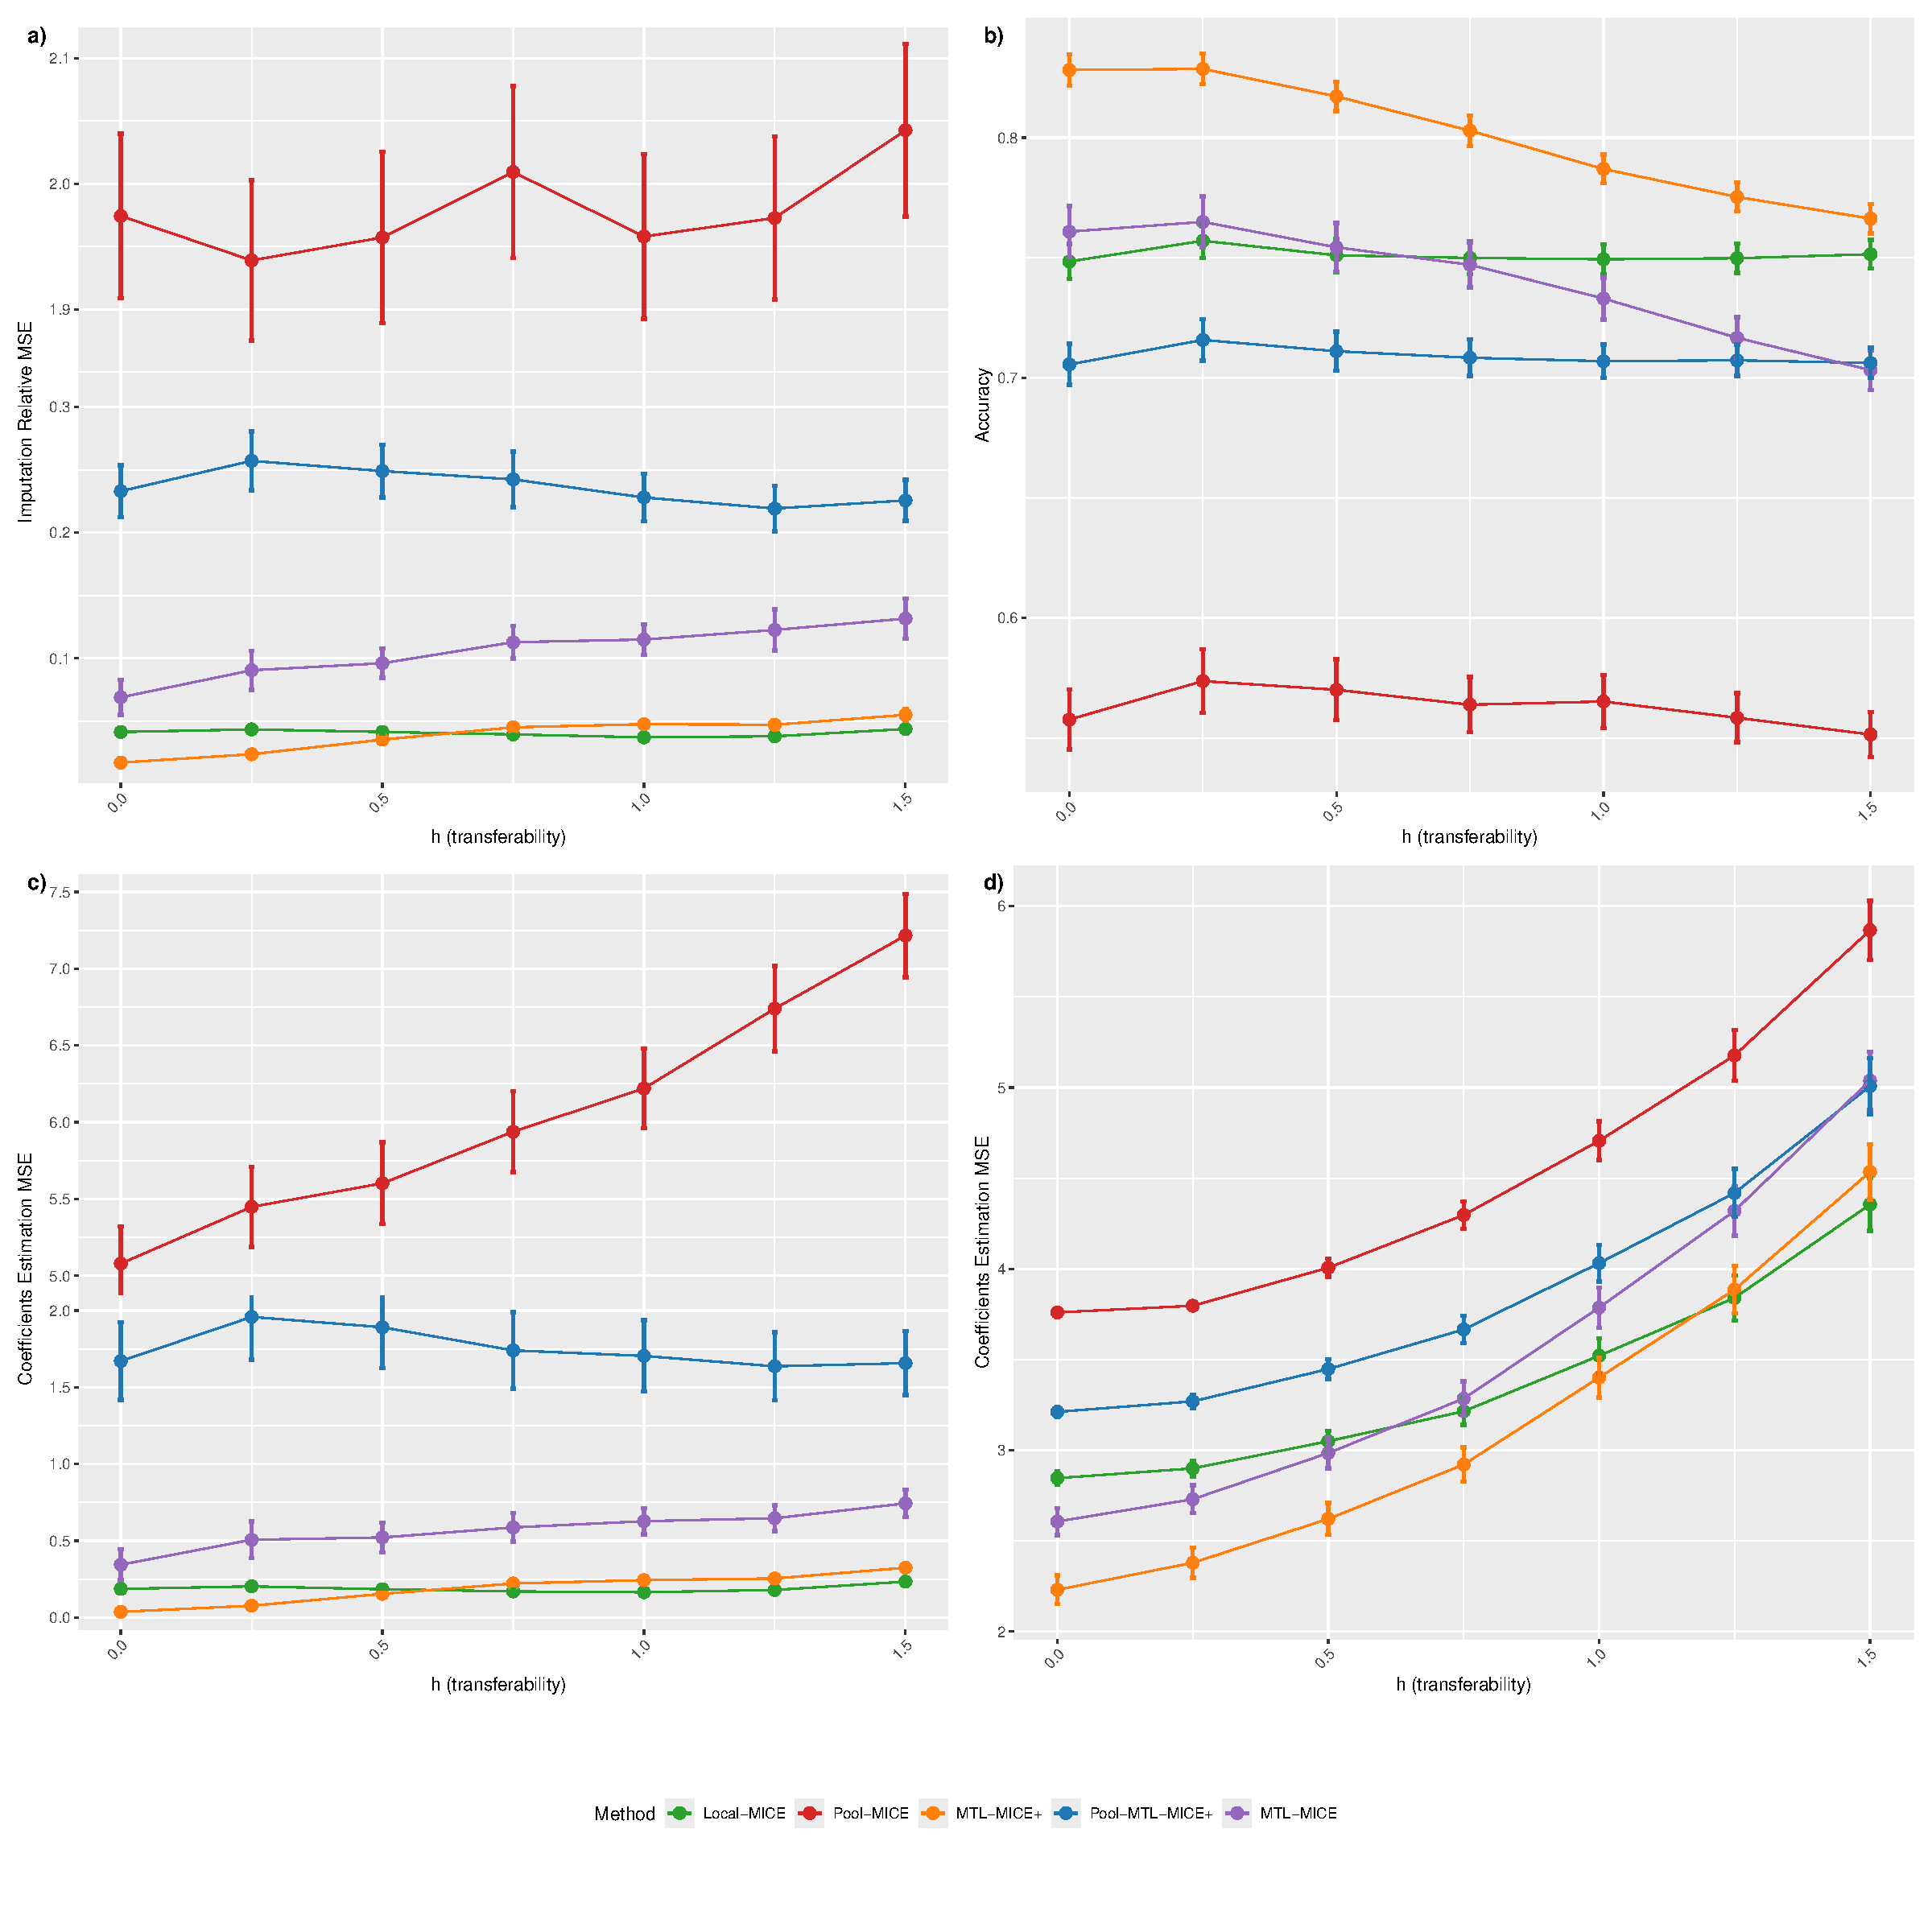
\includegraphics[width=1\linewidth]{plots/sim_htrends_cluster_combined_2x2_1se_2.pdf}

\caption{$h$-trend simulation with clustered tasks (Cluster 2 shown).
Tasks form two symmetric clusters of equal size with opposite coefficient baselines; therefore, Cluster 1 and Cluster 2 produce nearly identical performance curves, and we report Cluster 1 only.
Panels (a)–(b) summarize imputation performance as transferability decreases (larger $h$ implies weaker similarity within cluster), while panels (c)–(d) report coefficient recovery for the corresponding conditional models. Error bars show simulation uncertainty.}
\label{fig:htrend_cluster_2x2_cluster2}
\end{figure}

\begin{figure}[t]
\centering
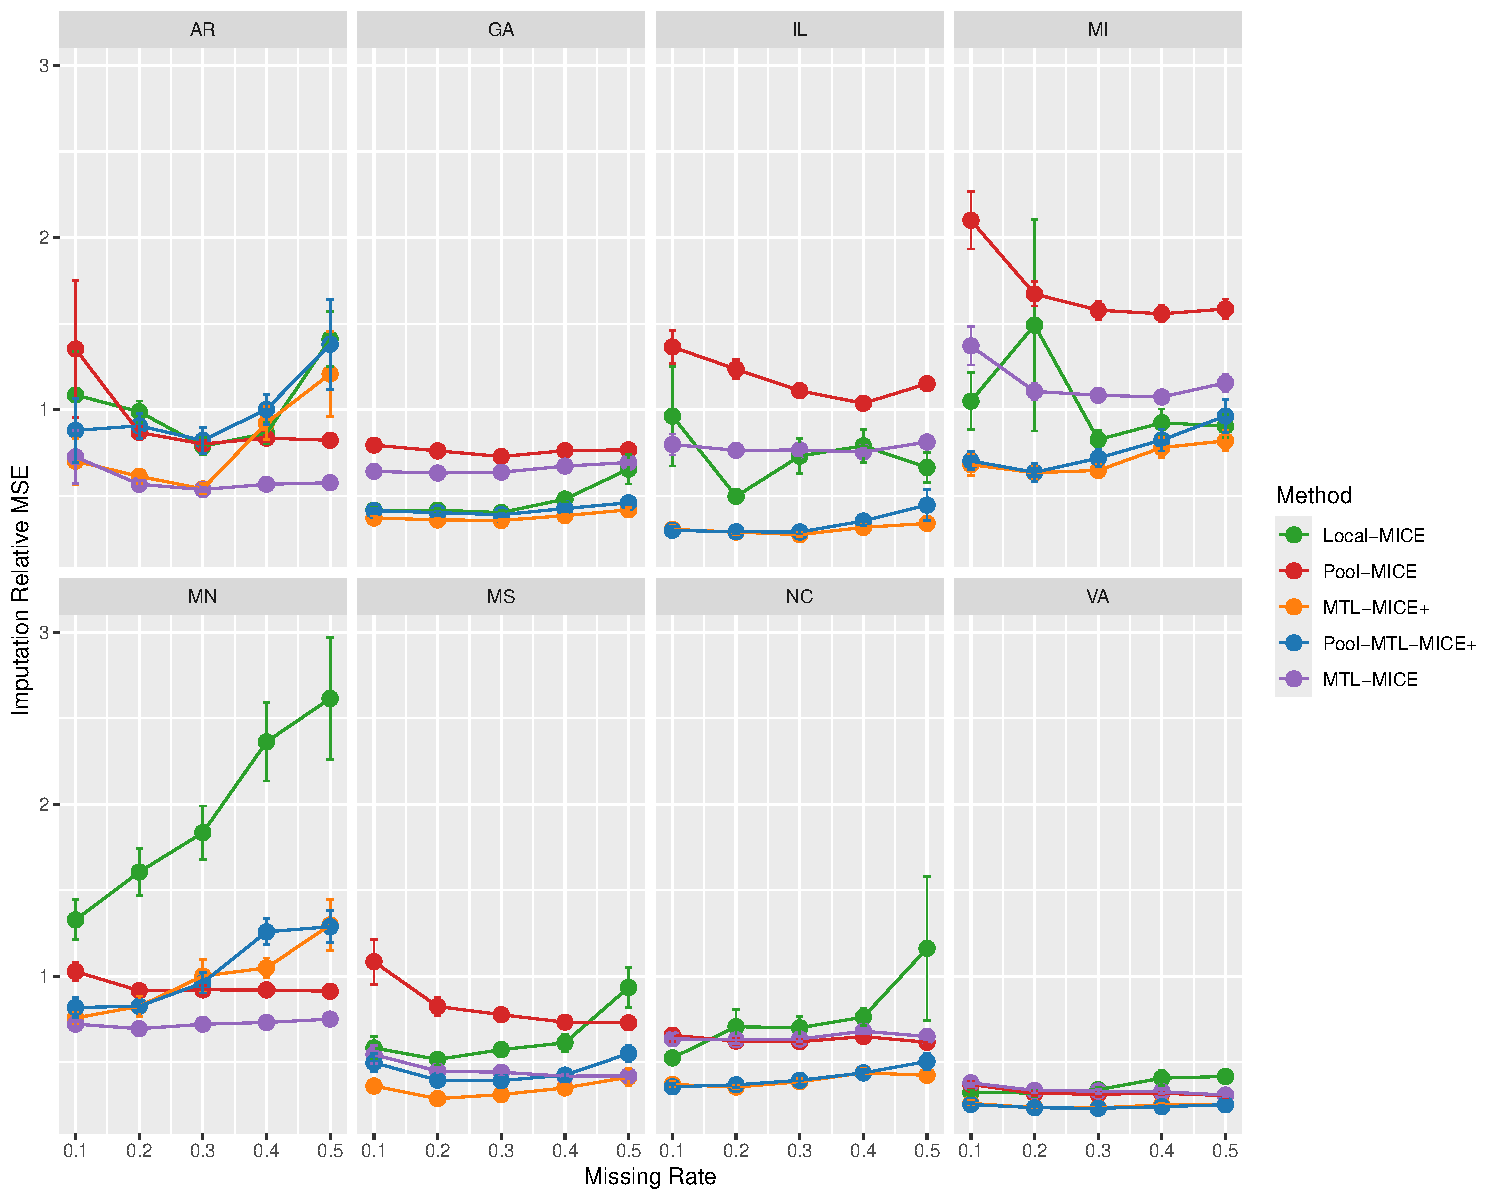
\includegraphics[width=1\linewidth]{plots/rda_uselection_continuous_rss_bystate_plot.pdf}
\caption{Real-data analysis (continuous, by state): county-level 2020 U.S.\ presidential election data.
States are treated as tasks and MAR missingness is introduced at rates
$\rho\in\{10\%,20\%,30\%,40\%,50\%\}$ (averaged over repeated masks).
The plot reports continuous imputation relative MSE, shown separately for each target state;
smaller values indicate better performance.}
\label{fig:rda_cont_bystate}
\end{figure}

\begin{figure}[t]
\centering
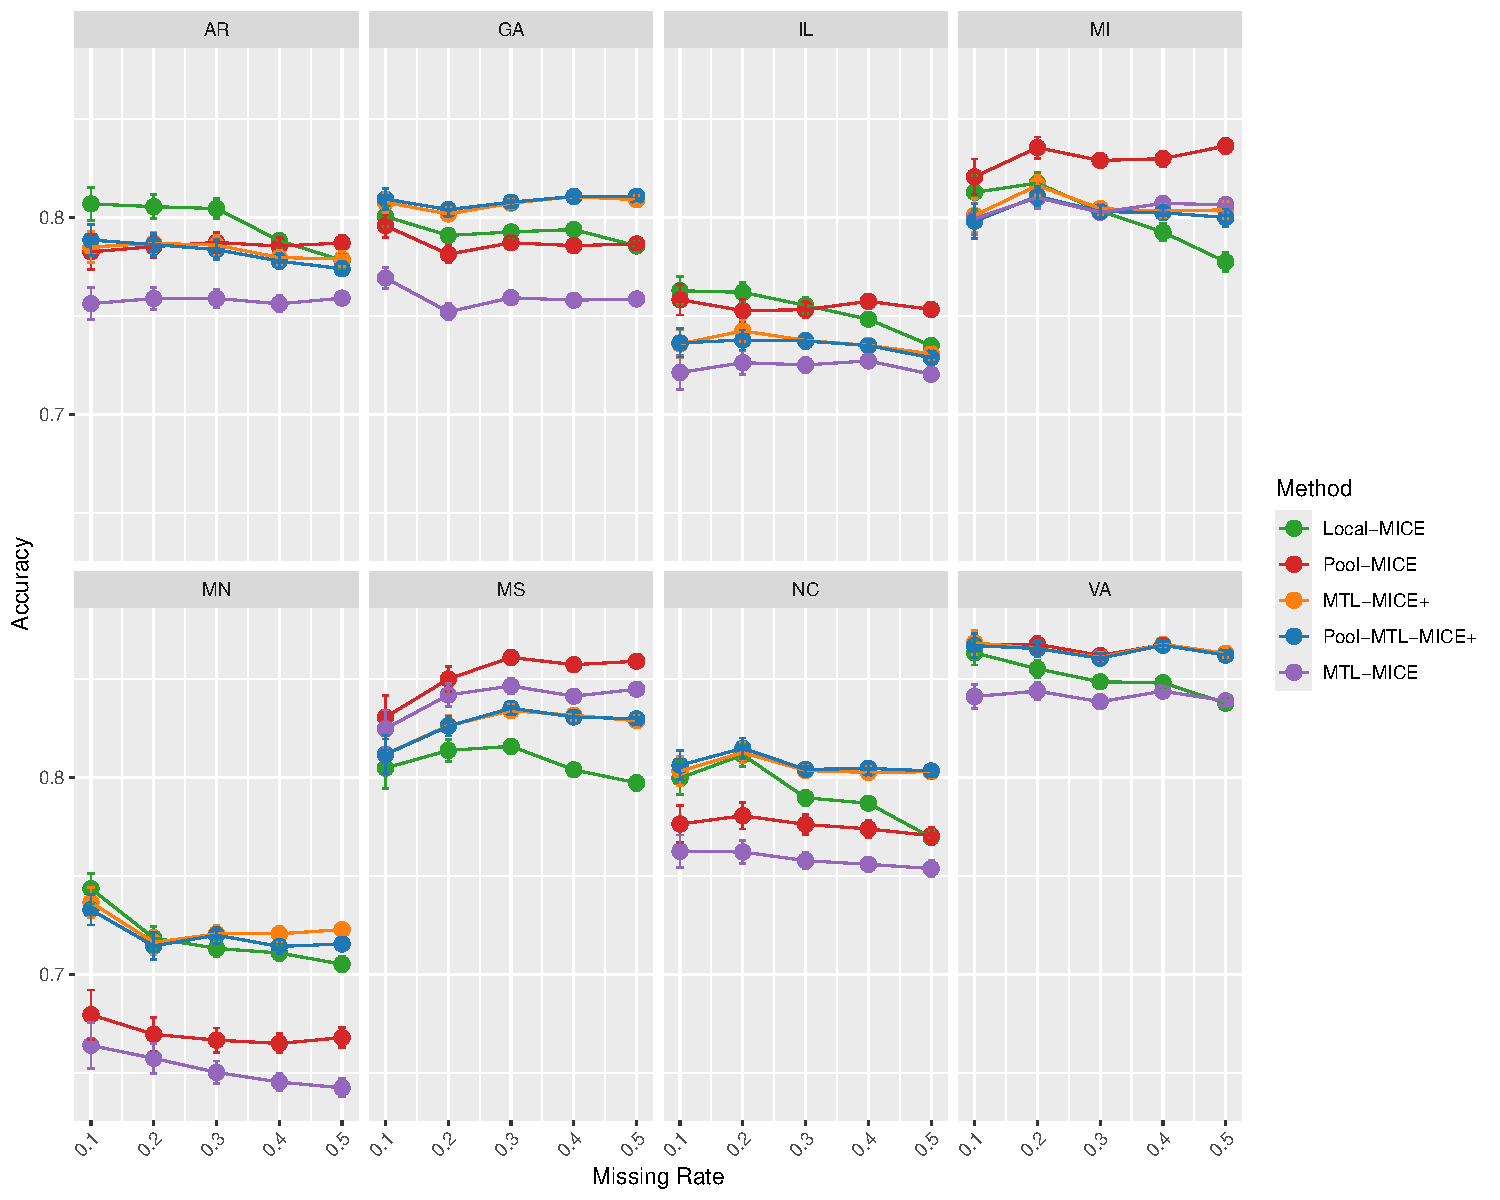
\includegraphics[width=1\linewidth]{plots/rda_uselection_categorical_bystate_plot.pdf}
\caption{Real-data analysis (binary, by state): county-level 2020 U.S.\ presidential election data.
States are treated as tasks and MAR missingness is introduced at rates
$\rho\in\{10\%,20\%,30\%,40\%,50\%\}$ (averaged over repeated masks).
The plot reports accuracy on masked cells for the binary variable (multi-unit housing $\ge 10\%$), shown separately for each target state;
larger values indicate better performance.}
\label{fig:rda_bin_bystate}
\end{figure}